% !TeX program = pdflatex
% !BIB program = biber



\addvspace{2\baselineskip plus 0.67\baselineskip}
% Because for some reason, \parnotes removes the vertical space before the following section heading

\section{Methods}
\label{sec:Methods}

In this section, we first present the design of the experiment (\ref{sec:design}) and derive behavioral predictions (\ref{sec:Predictions}).

\subsection{Design of the Main Experiment}
\label{sec:design}

\subsubsection{General Features}
\blindtext

\subsubsection{More Specific Features}
\blindtext

Let's test the euro symbol: \texteuro, \euro 1,234.56, $\euro 1{,}234.56$. Let's also test text superscripts: $i$\textsuperscript{th} and text subscripts: CO\textsubscript{2} and H\textsubscript{2}O.
$\sigma_\epsilon, c^\alpha$.
\blindtext
Let's test the footnote settings.\footnote{\blindmathfalse\blindtext\blindmathtrue} 

\begin{figure}[t]
	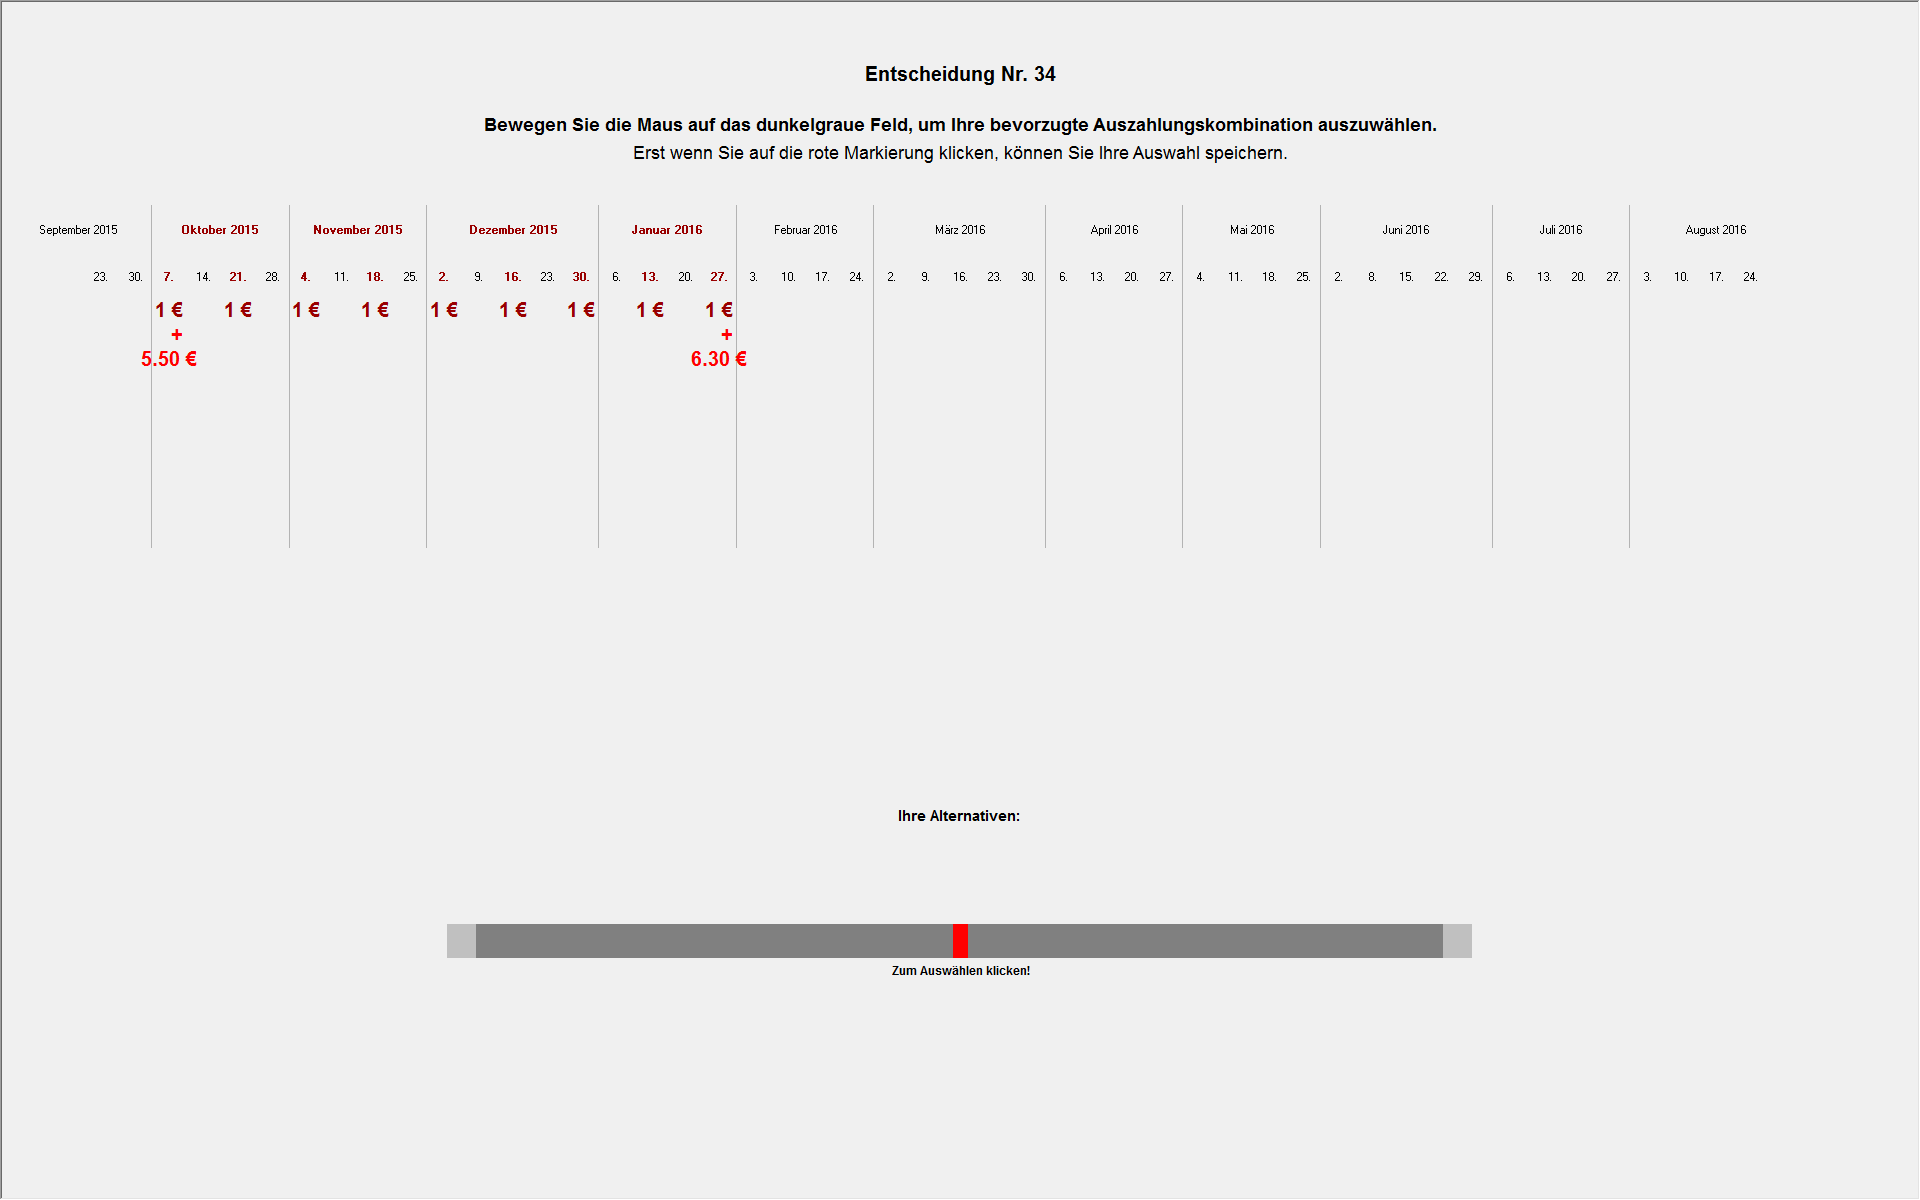
\includegraphics[width=\textwidth]{../figures/Screenshots/BS_inc_conc_half.png} \\[\medskipamount]
	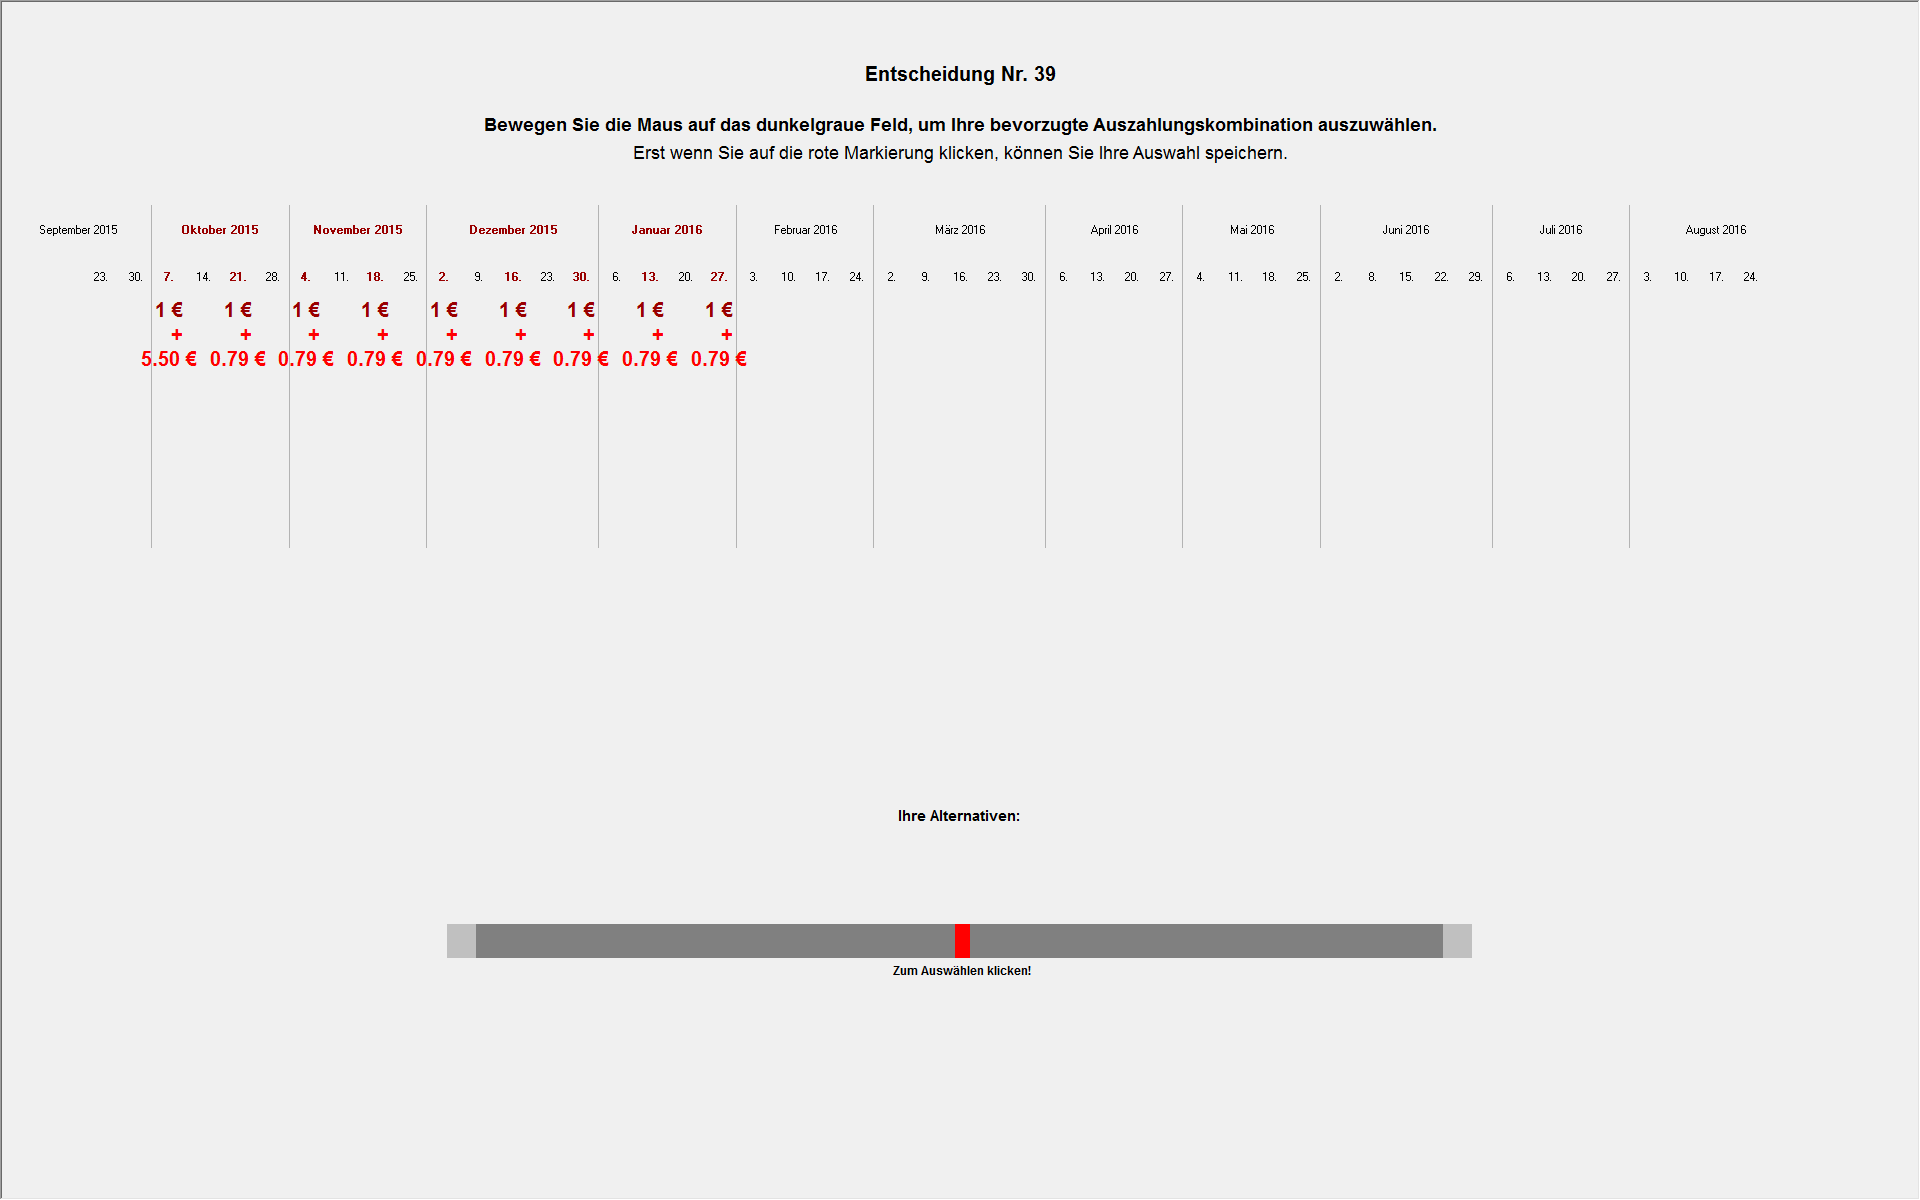
\includegraphics[width=\textwidth]{../figures/Screenshots/BS_inc_disp_half.png}
	\caption{Screenshots of a~\balA Decision (Top) and an~\unbalA[8] Decision (Bottom)%
	}
	\label{fig:screenshot:BS_inc_half}
	\figurenotes[Note:]{%
		This figure was taken from \cite{Dertwinkel-Kalt2017}.
	}
\end{figure}%

\autoref{fig:screenshot:BS_inc_half} shows an~exemplary decision screen with $B=\euro 11$ and $r\approx15\%$ for both \balA (upper panel) and \unbalA[8] (lower panel). Through a~slider, subjects choose their preferred ${x \in \CS[X]}$.\footnote{The slider had no initial position---it appeared only after subjects first positioned the mouse cursor over the slider bar. This was done to avoid default effects.} The slider position in Figure \ref{fig:screenshot:BS_inc_half} indicates ${x = 0.5}$, i.e., the earliest payment is reduced by \euro 5.50. Since ${r \approx 15\%}$ in this example, this slider position amounts to \euro 6.30 that are paid at later payment dates. While these \euro 6.30 are paid in a~single bank transfer on the latest payment date in \balA, the amount is dispersed in equal parts over the last 8~payment dates in \unbalA[8]---i.e., 8~consecutive payments of \euro 0.79.\footnote{We always rounded the second decimal place up so that the sum of the payments included in a~dispersed payoff was always at least as great as the respective concentrated payoff.}

\subsubsection{Some More Details}
\blindtext

Here's a~bulleted list:
\Blindlist{itemize}[3]
 
\subsubsection{Procedure}
\label{sec:Procedure}
Describe the sequence of events in your study. You could do this with the help of an~enumerated list:
\Blindlist{enumerate}[3]